\chapter{Allineamento di sequenze}
    Dopo aver esposto alcuni dei principali motivi per cui l'allineamento di sequenze risulta fondamentale nella \emph{bioinformatica}, si procede con una trattazione formale dell'argomento, partendo dal caso più semplice dell' \textbf{allineamento} di \textbf{due sequenze} fino ad arrivare a una sua generalizzazione tra un \textbf{grafo} e una \textbf{sequenza}. 
    
\section{Allineamento tra due sequenze}
    \textbf{Definizione}: Un \emph{allineamento} di due stringhe $S_1$ e $S_2$ si ottiene inserendo inizialmente gli \emph{spazi} (o \emph{indel}) all'inizio, all'interno o alla fine di $S_1$ e $S_2$, e successivamente allineando le due stringhe una sopra l'altra in maniera tale che, in entrambe le stringhe, ogni carattere o spazio risulti allineato a un singolo carattere o spazio dell'altra sequenza. Due spazi non possono risultare allineati tra loro. \cite{Gusfield}

    Un esempio di un allineamento delle due sequenze $S_1 = abbdcd$ e $S_2 = tbbqddc$ è il seguente:
    \vspace{20pt}
    \begin{table}[h]
        \centering
        \begin{tabular}{ccccccccc}
             a & - & b & b & - & d & c & d \\
             t & b & b & q & d & d & c & - \\
        \end{tabular}
    \end{table}
    \vspace{20pt}

    Una delle possibili metologie per approcciarsi al problema dell'allineamento è la \emph{programmazione dinamica}: infatti esso può essere visto come un \emph{problema di ottimizzazione}, descritto formalmente come segue:  
    
    \noindent
    \textbf{\textit{Input:}} 
    \begin{itemize}
        \item \textbf{Alfabeto} $\Sigma$
        \item \textbf{Sequenza} $X = <x_1, x_2, ..., x_n>, \, x_i \in \Sigma \quad \forall i \in \{1, ..., n\}$
        \item \textbf{Sequenza} $Y = <y_1, y_2, ..., y_m>, \, y_j \in \Sigma \quad \forall j \in \{1, ..., m\}$
        \item \textbf{Matrice di score} $d: (\Sigma \cup \{-\}) \times (\Sigma \cup \{-\}) \rightarrow \mathbb{Q}$
    \end{itemize}
    \textbf{\textit{Output:}} 
    \begin{itemize}
        \item \textbf{Valore dell'allineamento} $s = \sum_{i=1}^{k} d(x_i, y_i)$
    \end{itemize}

    In particolare, \emph{l'insieme delle soluzioni ammissibili} è composto da tutti i possibili allineamenti di $X$ e $Y$ (con eventualmente spazi inseriti all'inizio, all'interno o alla fine delle due stringhe); la \emph{soluzione ottimale} è quella che \emph{massimizza} il punteggio dell'allineamento (\textbf{massima omologia}).
    
\subsection{Equazioni di ricorrenza}
\label{section:needleman-wunsch}
\subsubsection{Dimostrazione di correttezza}
    Si considerino i prefissi delle due stringhe $X$ e $Y$
    \begin{itemize}
        \item $X_i = <x_1, x_2, ..., x_i>$,
        \item $Y_j = <y_1, y_2, ..., y_j>$
    \end{itemize}
    e sia $M[i, j]$ il \emph{valore ottimo} dell'allineamento di $X_{i}$ e $Y_{j}$; è possibile distinguere solo i seguenti casi:
    \begin{itemize}
        \item $x_i$ viene allineato con $y_j$: 
        \vspace{5pt}
        \begin{table}[h]
            \centering
            \begin{tabular}{|cccc|c|}
            \hline
                \multicolumn{4}{|c|}{$X_{i-1}$} & $X_i$\\
            \hline
                $x_0$ & $x_1$ & ... & $x_{i-1}$ & $x_i$ \\
                 $y_0$ & $y_1$ & ... & $y_{j-1}$ & $y_j$ \\
            \hline
                \multicolumn{4}{|c|}{$Y_{j-1}$} & $Y_j$\\
            \hline
            \end{tabular}
        \end{table}
        \vspace{5pt}
        
        in questo caso, il valore ottimo dell'allineamento sarà dato da
        $$M[i, j] = M[i-1, j-1] + d(x_i, y_j)$$
        
        \item $x_i$ viene allineato con '$-$': 
        \vspace{5pt}
        \begin{table}[h]
            \centering
            \begin{tabular}{|cccc|c|}
            \hline
                \multicolumn{4}{|c|}{$X_{i-1}$} & $X_i$\\
            \hline
                $x_0$ & $x_1$ & ... & $x_{i-1}$ & $x_i$ \\
                 $y_0$ & $y_1$ & ... & $y_{j-1}$ & $-$ \\
            \hline
                \multicolumn{4}{|c|}{$Y_{j-1}$} & \\
            \hline
            \end{tabular}
        \end{table}
        \vspace{5pt}
        
        in questo caso, il valore ottimo dell'allineamento sarà dato da
        $$M[i, j] = M[i-1, j] + d(x_i, -)$$
        \clearpage
        
        \item $y_j$ viene allineato con '$-$': 
        \vspace{5pt}
        \begin{table}[h]
            \centering
            \begin{tabular}{|cccc|c|}
            \hline
                \multicolumn{4}{|c|}{$X_{i-1}$} & \\
            \hline
                $x_0$ & $x_1$ & ... & $x_{i-1}$ & $-$ \\
                 $y_0$ & $y_1$ & ... & $y_{j-1}$ & $y_j$ \\
            \hline
                \multicolumn{4}{|c|}{$Y_{j-1}$} & $Y_j$\\
            \hline
            \end{tabular}
        \end{table}
        \vspace{5pt}
        
        in questo caso, il valore ottimo dell'allineamento sarà dato da
        $$M[i, j] = M[i, j-1] + d(-, y_j)$$
    \end{itemize}
    Non si riescono a individuare altre possibilità, quindi i tre casi elencati coprono tutte le casistiche; è possibile scrivere di conseguenza la seguente \emph{equazione di ricorrenza}:
    
    \vspace{20pt}
    \textbf{Needleman-Wunsch} \cite{NeedlemanWunsch}
    \begin{equation}
        M[i, j] = \max \begin{cases}
            M[i-1, j] + d(x_i, -) & \\
            M[i-1, j-1] + d(x_i, y_j) & \\
            M[i, j-1] + d(-, y_j) & \\
        \end{cases}
        \label{needleman-wunsch}
    \end{equation}
    $$\forall i > 0, \, \forall j > 0$$

\subsection{Ricostruzione della soluzione}
\label{subsection:traceback}
    Per ottenere anche l'allineamento effettivo delle due sequenze, è necessario salvare per ogni elemento di $M[i, j]$ la cella da cui è stato computato, in maniera da poter poi ricostruire la soluzione procedendo a ritroso. Formalmente, questo si traduce nel computare un'altra \emph{matrice di programmazione dinamica} di dimensione $(n + 1) \times (m + 1)$ come segue:
   \begin{equation}
        T[i, j] = \begin{cases}
            \uparrow, & se \, \, M[i, j] =  M[i-1, j] + d(x_i, -), \\
            \rotatebox[origin=c]{45}{$\uparrow$}, & se \, \, M[i, j] =  M[i-1, j-1] + d(x_i, y_j), \\
            \leftarrow, & se \, \, M[i, j] =  M[i, j-1] + d(-, y_j), \\
        \end{cases} \quad \forall (i, j) > \underline{0}
        \label{traceback}
    \end{equation}
\centering
    $$
        T[i, 0] = \, \, \uparrow \quad \forall i > 0
    $$
    $$
        T[0, j] = \, \, \leftarrow \quad \forall j > 0
    $$
    
\raggedright
    Una volta trovata la soluzione ottimale, è sufficiente seguire la sequenza delle celle salvate fino a $M[0, 0]$ per ricostruire l'allineamento.

\raggedright
\subsection{Complessità computazionale}
\label{section:needleman-wunsch_complexity}
\subsubsection{Complessità in tempo}
    Per calcolare l'allineamento ottimale, è necessario computare una matrice di dimensione $(n + 1) \times (m + 1)$, dove ogni elemento viene calcolato in $\Theta(1)$ (equazioni \ref{needleman-wunsch} e \ref{traceback}); di conseguenza, la \emph{complessità temporale} dell'algoritmo sarà data da:
    \begin{equation*}
        T(n, m) = \Theta(nm)
    \end{equation*}

    Per ricostruire la soluzione, invece, è necessario ripercorrere a ritroso il percorso ottimale all'interno della matrice; nel caso migliore questo significa muoversi sempre in diagonale fino alla cella iniziale, mentre nel caso peggiore si seguirà un percorso composto unicamente da passi orizzontali e verticali. In ogni caso, la complessità risulta minore della computazione della matrice: nel \textbf{caso migliore} è \emph{limitata inferiormente} da
    \begin{equation*}
        T(n, m) = \Omega(\max\{n, m\})
    \end{equation*}
    mentre nel \textbf{caso peggiore} risulta \emph{limitata superiormente} da
    \begin{equation*}
        T(n, m) = O(n + m)
    \end{equation*}
    
\subsubsection{Complessità in spazio}
    Ogni elemento della matrice occupa una quantità di memoria \emph{costante}, quindi, in maniera analoga, la \emph{complessità spaziale}\footnote{Se si è interessati solo al \emph{valore dell'allineamento} e non alla \emph{ricostruzione della soluzione}, non è necessario salvare tutta la matrice, ma basta mantenere una sola riga (o colonna, a seconda di come la si computa) per volta. La \textbf{complessità spaziale} risulta quindi $\Theta(\min \{n, m \})$.} sarà:
    \begin{equation*}
        M(n, m) = \Theta(nm)
    \end{equation*}

\subsection{Caso globale}
\subsubsection{Condizioni al contorno}
    
    Nel \textbf{caso globale}, l'obiettivo è quello di allineare completamente le due stringhe: come conseguenza, l'allineamento deve inizare dal primo simbolo e finire all'ultimo, per entrambe le sequenze. Formalmente, questo si traduce nelle seguenti \emph{condizioni al contorno}:

    \begin{equation}
        M[i, j] = \begin{cases}
            0 & i = 0, j = 0 \\
            M[i-1, 0] + d(x_i, -) & i > 0, j = 0\\
            M[0, j-1] + d(-, y_j) & i = 0, j > 0\\
        \end{cases}
    \end{equation}

    La \textbf{soluzione ottima} è data dall'allineamento di entrambe le sequenze nella loro interezza: 
    \begin{equation}
        s = M[n, m]
    \end{equation}
    
\subsubsection{Esempio}
    Di seguito un esempio dell'\textbf{allineamento globale} ottimale di due sequenze nucletotidiche:
    
    \vspace{20pt}
    \noindent \textbf{\textit{Input}}
    \begin{itemize}
        \item $\Sigma$ = \{A, G, C, T\} 
        \item $X$ = "GAATTCAGTTA"
        \item $Y$ = "GGATCGA"
        \item $d(x, y) = \begin{cases}
            5 & \forall x, y \in \Sigma \mid x = y, \\
            -3 & \forall x, y \in \Sigma \mid x \neq y, \\
            -4 & \forall x \in \Sigma, y = -, \\
            -4 & x = -, \forall y \in \Sigma
        \end{cases}$
    \end{itemize}
    
    \noindent
    \textbf{\textit{Output}}
    
    \centering \textbf{Score} = 11
    \vspace{20pt}
    \begin{table}[h]
        \centering
        \begin{tabular}{ccccccccccc}
             G & A & A & T & T & C & A & G & T & T & A \\
             | &   & | &   & | & | &   & | &   &   & | \\
             G & G & A & - & T & C & - & G & - & - & A \\
             \hline
             +5 & -3 & +5 & -4 & +5 & +5 & -4 & +5 & -4 & -4 & +5 \\
             \hline
        \end{tabular}
    \end{table}
    \vspace{20pt}

\raggedright
\subsection{Caso semiglobale}
\subsubsection{Condizioni al contorno}

    Nel \textbf{caso semiglobale}, la seconda sequenza (chiamata solitamente \emph{query} o \emph{read}) può essere allineata a una qualsiasi \emph{sottostringa} della prima (chiamata \emph{testo}): in altre parole, è possibile inserire un numero qualsiasi di \emph{spazi} all'inizio e alla fine della \emph{read} senza penalità aggiuntive. Definita quindi $X$ come la \textbf{sequenza di riferimento} e $Y$ come la \textbf{query} da allineare, questo si traduce nelle seguenti \emph{condizioni al contorno}:

    \begin{equation}
        M[i, j] = \begin{cases}
            0 & i \geq 0, j = 0 \\
            M[0, j - 1] + d(-, y_j) & i = 0, j > 0 \\
        \end{cases}
    \end{equation}

    La \textbf{soluzione ottima} sarà data dall'allineamento che comprende tutta la \emph{read} e una qualsiasi sottostringa del \emph{testo} e che \emph{massimizza il punteggio}, ovvero: 
    \begin{equation}
        s = \max_{0 \leq i \leq n} M[i, m]
    \end{equation}
    
\subsubsection{Esempio}
    Di seguito un esempio dell'\textbf{allineamento semiglobale} ottimale di due sequenze nucletotidiche:

    \vspace{20pt}
    \noindent \textbf{\textit{Input}}
    \begin{itemize}
        \item $\Sigma$ = \{A, G, C, T\} 
        \item $X$ = "GAATTCAGTTA"
        \item $Y$ = "AAACGGT"
        \item $d(x, y) = \begin{cases}
            5 & \forall x, y \in \Sigma \mid x = y, \\
            -3 & \forall x, y \in \Sigma \mid x \neq y, \\
            -4 & \forall x \in \Sigma, y = -, \\
            -4 & x = -, \forall y \in \Sigma
        \end{cases}$
    \end{itemize}

    \noindent \textbf{\textit{Output}}
    
\centering 
    \textbf{Score} = 23
    \vspace{20pt}
    \begin{table}[h]
        \centering
        \begin{tabular}{ccccccccccc}
             G & A & A & T & T & C & G & G & T & T & A \\
               & | & | &   &   & | & | & | & | &   &  \\
             - & A & A & - & A & C & G & G & T & - & - \\
             \hline
             0 & +5 & +5 & -4 & -3 & +5 & +5 & +5 & +5 & 0 & 0 \\
             \hline
        \end{tabular}
    \end{table}
    \vspace{20pt}

\raggedright
\section{Distanza di edit tra due sequenze}
\label{section:edit-distance}
    Un'altra possibilità per misurare quanto due sequenze sono simili tra loro è calcolare la \textbf{distanza} che le divide; in particolare, ci sono numerose maniere con cui viene formalizzata la \emph{distanza tra due stringhe}: una delle più utilizzate è la \textbf{\textit{distanza di edit}}, la quale fornisce il minimo numero di operazioni necessarie a trasformare una stringa nell'altra (oltre all'effettiva sequenza di operazioni necessarie).
    \vspace{20pt}
    
    \textbf{Definizione}: La \emph{distanza di edit} tra due sequenze è definita come il \emph{minimo} numero di \emph{operazioni di edit} - \textbf{inserimenti, cancellazioni e sostituzioni} - necessarie a trasformare la prima sequenza nella seconda. \cite{Gusfield}
    \vspace{20pt}
    
    Si noti che la \textbf{distanza di edit} riferita alla trasformazione della prima sequenza nella seconda è sempre uguale a quella che si riferisce alla trasformazione opposta: è inoltre possibile passare da un \textbf{edit transcript} al duale semplicemente invertendo le operazioni effettuate.

    In maniera analoga all'\textbf{allineamento di sequenze}, anche il problema della \textbf{distanza di edit} può essere risolto in maniera efficiente tramite \emph{programmazione dinamica}:
    \vspace{20pt}
    
    \noindent \textbf{\textit{Input:}} 
    \begin{itemize}
        \item \textbf{Alfabeto} $\Sigma$
        \item \textbf{Sequenza} $X = <x_1, x_2, ..., x_n>, \, x_i \in \Sigma \quad \forall i \in \{1, ..., n\}$
        \item \textbf{Sequenza} $Y = <y_1, y_2, ..., y_m>, \, y_j \in \Sigma \quad \forall j \in \{1, ..., m\}$
    \end{itemize}
    \textbf{\textit{Output:}} 
    \begin{itemize}
        \item \textbf{Distanza di edit} $d$
        \item \textbf{Sequenza} delle \textbf{operazioni di edit} (\textbf{edit transcript})
    \end{itemize}

    \emph{L'insieme delle soluzioni ammissibili} è composto da tutte gli \textbf{edit transcript} che trasformano $X$ in $Y$; la \emph{soluzione ottimale} è quella che minimizza il numero delle \emph{operazioni di edit}.
    
\subsection{Equazioni di ricorrenza}
\subsubsection{Dimostrazione di correttezza}
    Si considerino i prefissi delle due stringhe $X_i = <x_1, x_2, ..., x_i>$, $Y_j = <y_1, y_2, ..., y_j>$ e siano noti
    \begin{itemize}
        \item $D[i, j]$, il \emph{valore ottimo} della distanza di edit tra $X_{i}$ e $Y_{j}$;
        \item $S[i, j]$, l'insieme delle \emph{operazioni di edit} per trasformare $X_i$ in $Y_j$;
    \end{itemize} è possibile distinguere 4 casistiche\footnote{Le \emph{operazioni di edit} sono rapprentate come \begin{itemize}
        \item $I(a)$: $a$ viene inserito nella sequenza;
        \item $M(a, b)$: $a$ viene sostituito da $b$ nella sequenza;
        \item $D(b)$: $b$ viene cancellato dalla sequenza.
    \end{itemize}}:
    \begin{itemize}
        \item $x_i = y_j$: in questo caso nessuna operazione è necessaria e la \emph{distanza di edit} resta invariata:
            $$D[i + 1, j + 1] = D[i, j]$$
            $$S[i + 1, j + 1] = S[i,j]$$ 
        
        \item $x_i \neq y_j$: in questo caso ci sono 3 possibilità: 
        \begin{itemize}
            \item \textbf{Inserimento}, ovvero $y_j$ viene aggiunto alla sequenza $X_i$: in questo caso la \emph{distanza di edit} aumenta di uno:
            $$D[i, j + 1] = D[i, j] + 1$$
            $$S[i, j + 1] = S[i, j] \cup I(y_j)$$

            \item \textbf{Sostituzione}, ovvero $x_i$ viene sostituito con $y_j$: in questo caso la \emph{distanza di edit} aumenta di uno:
            $$D[i + 1, j + 1] = D[i, j] + 1$$
            $$S[i + 1, j + 1] = S[i, j] \cup M(x_i, y_j)$$

            \item \textbf{Cancellazione}, ovvero $x_i$ viene cancellato dalla sequenza $X_i$: in questo caso la \emph{distanza di edit} aumenta di uno:
            $$D[i + 1, j] = D[i, j] + 1$$
            $$S[i + 1, j] = S[i, j] \cup D(x_i)$$
        \end{itemize}
    \end{itemize}
        
    Non esistono altre possibilità, quindi i quattro casi elencati coprono tutte le casistiche; è possibile scrivere di conseguenza la seguente \emph{equazione di ricorrenza}
    \begin{equation}
        D[i, j] = \begin{cases}
            D[i-1, j-1] & se \, \, x_i = y_j \\
            \min \begin{cases}
                D[i, j-1] & \\
                D[i-1, j-1] & \\
                D[i-1, j] & \\
            \end{cases} + 1 & se \, \, x_i \neq y_j 
        \end{cases}
        \label{edit-distance}
    \end{equation}
\centering
    $\forall i > 0, \, \forall j > 0$
    
\raggedright
    Insieme alle seguenti \emph{condizioni al contorno}
    \begin{equation}
        D[i, j] = \begin{cases}
            0 & i = 0, j = 0 \\
            D[0, j-1] + 1 & i = 0, j > 0 \\
            D[i-1, 0] + 1 & i > 0, j = 0 \\
        \end{cases}
    \label{edit-distance-base-case}
    \end{equation}

    La \emph{distanza di edit ottimale} è data da $D[n, m]$.

\subsection{Ricostruzione della soluzione}
    Per la sequenza delle \emph{operazioni di edit} si procede come per l'allineamento di sequenze (sezione \ref{subsection:traceback}), salvando per ogni elemento di $D[i, j]$ la cella da cui è stato computato, in maniera da poter poi ricostruire la soluzione procedendo all'indietro.
    
\raggedright
\subsection{Complessità computazionale}
\subsubsection{Complessità in tempo}
    Per calcolare l'allineamento ottimale, è necessario computare una matrice di dimensione $(n + 1) \times (m + 1)$, dove ogni elemento viene calcolato in $\Theta(1)$ (equazione \ref{edit-distance}); di conseguenza, la \emph{complessità in tempo} dell'algoritmo sarà data da:
    \begin{equation*}
        T(n, m) = \Theta(nm)
    \end{equation*}

    Come per l'\textbf{allineamento di sequenze} (sezione \ref{section:needleman-wunsch_complexity}), la ricostruzione della soluzione è per la \textbf{distanza di edit} è \emph{limitata superiormente} da
    \begin{equation*}
        T(n, m) = O(n + m)
    \end{equation*}
    
\subsubsection{Complessità in spazio}
    Ogni elemento della matrice occupa una quantità di memoria \emph{costante}, quindi, in maniera analoga, la \emph{complessità spaziale}\footnote{Se si è interessati solo alla \emph{distanza di edit} e non alla \emph{sequenza di operazioni di edit}, non è necessario salvare tutta la matrice, ma basta mantenere una sola riga (o colonna, a seconda di come la si computa) per volta. La \textbf{complessità spaziale} risulta quindi $\Theta(\min \{n, m \})$.} sarà:
    \begin{equation*}
        M(n, m) = \Theta(nm)
    \end{equation*}

\subsection{Caso pesato}
    E' possibile estendere il problema della \emph{distanza di edit} a considerare penalità per le diverse operazioni non unitarie (e non necessariamente uguali), mantenendo comunque la \emph{stessa complessità}. Si introducono
    \begin{itemize}
        \item \textbf{\textit{i}} = penalità per un \emph{inserimento},
        \item \textbf{\textit{m}} = penalità per una \emph{sostituzione},
        \item \textbf{\textit{d}} = penalità per una \emph{cancellazione},
    \end{itemize}
    con $(i, m, d) \in \mathbb{Q}^3_+$; è possibile riscrivere le equazioni \ref{edit-distance} e \ref{edit-distance-base-case} come:

    \begin{equation}
        D[i, j] = \begin{cases}
            D[i-1, j-1] & se \, \, x_i = y_j \\
            \min \begin{cases}
                D[i, j-1] + i & \\
                D[i-1, j-1] + m & \\
                D[i-1, j] + d & \\
            \end{cases} & se \, \, x_i \neq y_j 
        \end{cases}
        \label{edit-distance-weighted}
    \end{equation}
\centering
    $\forall i > 0, \, \forall j > 0$
    
    \begin{equation}
        D[i, j] = \begin{cases}
            0 & i = 0, j = 0 \\
            D[0, j-1] + i & i = 0, j > 0 \\
            D[i-1, 0] + d & i > 0, j = 0 \\
        \end{cases}
        \label{edit-distance-weighted-base-case}
    \end{equation}

\raggedright
\subsubsection{Esempio}
    Di seguito un esempio del calcolo della \textbf{distanza di edit pesata} di due sequenze nucletotidiche:
    
    \vspace{20pt}
    \noindent \textbf{\textit{Input}}
    \begin{itemize}
        \item $\Sigma$ = \{A, G, C, T\} 
        \item $X$ = "GAATTCAGTTA"
        \item $Y$ = "GGATCGA"
        \item $i$ = 4
        \item $m$ = 3
        \item $d$ = 4
    \end{itemize}
    
    \noindent
    \textbf{\textit{Output}}
    
    \centering \textbf{Weighted edit distance} = 19
    \vspace{20pt}
    \begin{table}[h]
        \centering
        \begin{tabular}{ccccccccccc}
             G & A & A & T & T & C & A & G & T & T & A \\
             | & | & | & $d$ & | & | & $d$ & | & $d$ & $d$ & | \\
             G & A & A &   & T & C &   & G &   &   & A \\
             | & $m$ & | &  & | & | &  & | &  &  & | \\
             G & G & A &   & T & C &   & G &   &   & A \\
             \hline
             0 & 3 & 0 & 4 & 0 & 0 & 4 & 0 & 4 & 4 & 0 \\
             \hline
        \end{tabular}
    \end{table}
    \vspace{20pt}

\raggedright
\section{Estensione all'allineamento tra un grafo e una sequenza}
    I \textbf{grafi di pangenomi} sono strutture che rappresentano una collezione di \emph{genomi} e codificano variazioni di sequenze al loro interno, permettendo lo studio di più genomi simili tra loro. Per riuscire a utilizzare queste strutture risulta necessario generalizzare il problema dell'allineamento: di seguito vengono riportate due estensioni a riguardo, rispettivamente su \textbf{grafi di sequenza} e \textbf{grafi di variazione}.
    
\subsection{Grafi di sequenza}
    Un \textbf{grafo di sequenza} (o \textbf{sequence graph}) è una struttura dati utilizzata per rappresentare e analizzare le relazioni tra sequenze di DNA, RNA o proteine; i nodi rappresentano le diverse sequenze e gli archi rappresentano le relazioni tra di esse. Gli archi possono indicare la presenza di varianti, come mutazioni, inserzioni o delezioni, che possono differire tra le diverse sequenze rappresentate nel grafo. Formalmente, un \textbf{sequence graph} si definisce come segue:
    
    \vspace{20pt}
    \textbf{Definizione:} un \emph{sequence graph} è una tripla $G = (V, E, \delta)$, dove
    \begin{itemize}
        \item $V = \{v_1, v_2, ..., v_n\}$ è l'insieme dei \textbf{vertici} del grafo, che rappresentano le sequenze;
        \item  $E \subseteq V \times V$ è l'insieme degli \textbf{archi} del grafo, che rappresentano le relazioni tra diverse sequenze;
        \item $\delta: V \rightarrow \Sigma^*$ è la \textbf{funzione di etichettatura}, che associa a ogni vertice la sequenza corrispondente.
    \end{itemize}
    In particolare, se a ogni \textbf{vertice} viene associato un solo carattere (e quindi la \textbf{funzione di etichettatura} è definita come $\delta: V \rightarrow \Sigma$), il \emph{grafo} viene detto \emph{canonico}. 

    \vspace{10pt}
    \begin{figure}[h]
        \centering
        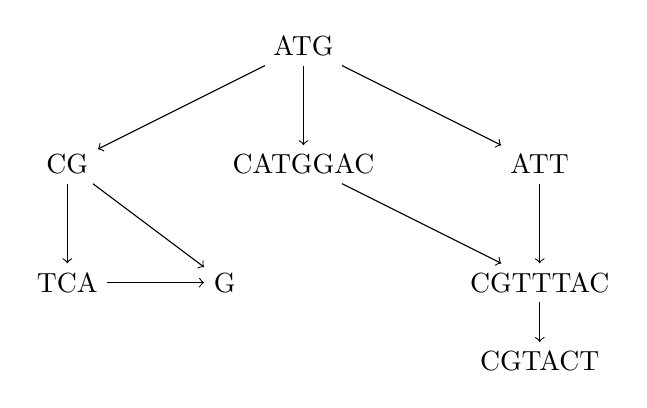
\begin{tikzpicture}
              % Nodi
              \node (1) at (5,0) {ATG};
              \node (2) at (2,-1.5) {CG};
              \node (3) at (8,-1.5) {ATT};
              \node (4) at (2,-3) {TCA};
              \node (5) at (4,-3) {G};
              \node (6) at (8,-3) {CGTTTAC};
              \node (7) at (8,-4) {CGTACT};
              \node (8) at (5, -1.5) {CATGGAC};
            
              % Archi
              \draw[->] (1) -- (2);
              \draw[->] (1) -- (3);
              \draw[->] (1) -- (8);
              \draw[->] (8) -- (6);
              \draw[->] (2) -- (4);
              \draw[->] (2) -- (5);
              \draw[->] (3) -- (6);
              \draw[->] (6) -- (7);
              \draw[->] (4) -- (5);
            \label{graph:sequence-graph}
        \end{tikzpicture}
        \caption{Esempio di \textbf{grafo di sequenza}.}
    \end{figure}

\subsection{Partial Order Alignment (POA)}
    Una delle possibilità per rappresentare un \emph{allineamento multiplo di sequenze} è tramite una struttura chiamata \textbf{POA (Partial Order Alignment)} \cite{POA}, che utilizza un \textbf{grafo di sequenza} \emph{ordinato topologicamente} per rappresentare l'allineamento. Nella figura \ref{fig:poa_construction} è riportato un esempio:
    \clearpage

    \begin{figure}[ht]
        \centering
        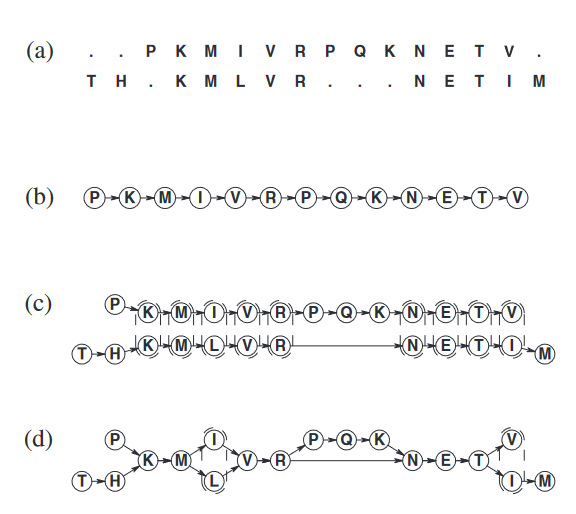
\includegraphics{images/poa-construction.png}
        \caption{\textbf{MSA} rappresentato con un \textbf{POA}. (a) Rappresentazione in formato \textbf{RC-MSA} di un allineamento di sequenze proteiche. (b) Una singola sequenza in formato \textbf{PO-MSA}. (c) Due sequenze proteiche allineate tra loro in formato \textbf{PO-MSA}. I cerchi tratteggiati indicano che due nodi sono allineati. (d) Rappresentazione in formato \textbf{PO-MSA} di un allineamento di due sequenze proteiche. I cerchi tratteggiati indicano che due nodi sono allineati. \cite{POA}}
        \label{fig:poa_construction}
    \end{figure}

\subsubsection{Allineamento tra un POA e una sequenza}
    L'algoritmo di \textbf{programmazione dinamica} \textbf{Needleman-Wunsch} per calcolare l'allineamento tra sequenze (sezione \ref{section:needleman-wunsch}) può essere esteso in maniera da funzionare anche su \textbf{ordini parziali}. In maniera informale, è possibile considerare una sequenza come un grafo degenere, in cui ogni vertice (tranne il primo e l'ultimo) hanno esattamente un predecessore e un successore: per estendere \textbf{Needleman-Wunsch} all'utilizzo di \textbf{POA}, è sufficiente che per ogni vertice non si consideri solo un nodo precedente, bensì tutti i predecessori di tale vertice. Formalmente, considerati in ingresso
    \begin{itemize}
        \item un \textbf{alfabeto} $\Sigma$,
        \item un \textbf{grafo canonico} $G = (V, E, \delta)$ con 
        \begin{itemize}
            \item $V = \{v_1, v_2, ..., v_n\}$ \textbf{ordinato topologicamente}, a cui si aggiunge un vertice $v_0$ per rappresentare il \textbf{grafo vuoto},
            \item $E : V \times V$, a cui si aggiunge $(v_0, v_1)$,
            \item $\delta: V \rightarrow \Sigma$, a cui si aggiunge $\delta(v_0) = \epsilon$,
        \end{itemize}
        \item una \textbf{sequenza (o read)} $X = <x_1, x_2, ..., x_m>, \, x_j \in \Sigma \, \, \forall j \in \{1, 2, ..., m\}$,
        \item una \textbf{matrice di score} $d : (\Sigma \cup \{-\}) \times (\Sigma \cup \{-\}) \rightarrow \mathbb{Q}$
    \end{itemize}
    questo si traduce nella seguente \emph{equazione di ricorrenza}:

    \begin{equation}
        M[v, j] = \max \begin{cases}
            M[u, j] + d(\delta(v), -) & \\
            M[u, j - 1] + d(\delta(v), x_j) & \\
            M[v, j - 1] + d(-, x_j) & \\
        \end{cases}
    \label{equation:poa}
    \end{equation}
    $$\forall u \, s.t. \, (u,v) \in E, \, \forall j > 0 $$

    e nelle seguenti \emph{condizioni al contorno}:
\subsubsection{Caso globale}
    \textbf{Caso base}:
    \begin{equation}
        M[v, j] = \begin{cases}
            0 & v = v_0, \, j = 0 \\
            M[u, 0] + d(\delta(u), -)& \forall (u, v) \in E, \, j = 0 \\
            M[v_0, j - 1] + d(-, x_j)& v = v_0, \, j > 0
        \end{cases}
    \end{equation}

    \textbf{Soluzione ottima}: $$M[v_n, m]$$
    
\subsubsection{Caso semiglobale}
    \textbf{Caso base}:
    \begin{equation}
        M[v, j] = \begin{cases}
            0 & \forall v \in V, \, j = 0 \\
            M[v_0, j - 1] + d(-, x_j) & v = v_0, \, j > 0
        \end{cases}
    \end{equation}
    \textbf{Soluzione ottima}:
    $$\max_{v \in V} M[v, m]$$

\clearpage
\subsubsection{Esempio}
    Come esempio si propone una visualizzazione grafica della \emph{matrice di programmazione dinamica} costruita tramite l'algoritmo appena descritto:
    \begin{figure}[ht]
        \centering
        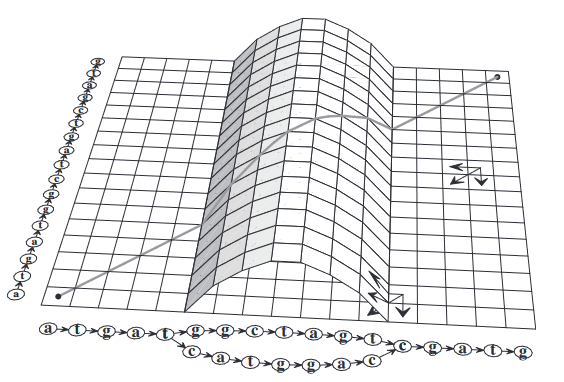
\includegraphics{images/poa-example.png}
        \caption{\emph{Matrice di prgrammazione dinamica} di un allineamento tra un \textbf{POA} e una \textbf{sequenza}. \cite{POA}}
        \label{fig:poa_example}
    \end{figure}
    
    \vspace{20pt}
    Come si vede dalla figura \ref{fig:poa_example}, da ogni \textbf{vertice} con \emph{successori multipli} viene computata una nuova \emph{matrice di programmazione dinamica}; in maniera analoga, in ogni \textbf{nodo} con \emph{più di un predecessore}, due diverse \emph{matrici} si fondono in una sola.  

\subsubsection{Complessità computazionale}
\label{section:poa-complexity}
    Come nell' \textbf{allineamento di sequenze} (sezione \ref{section:needleman-wunsch_complexity}), è necessario computare una matrice di dimensione $(n + 1) \times (m+1)$; la differenza risiede nel fatto che ogni elemento della matrice non è più computabile da un \emph{numero finito} di \emph{casi}, bensì dipende dal numero di \emph{predecessori} di ogni vertice (equazione \ref{equation:poa}): di conseguenza, non è più possibile considerare \emph{costante} il tempo con cui calcola ogni cella. Quindi, definito
    \begin{itemize}
        \item $\bar{n_p}$ = \emph{numero medio} di \emph{predecessori} per vertice
    \end{itemize}
    La \textbf{complessita in tempo} dell'algoritmo risulta essere
    \begin{equation*}
        T(n, m) = \Theta((2\bar{n_p} + 1) \cdot n \cdot m) = \Theta(\bar{n_p} \cdot n \cdot m)
    \end{equation*}
    lineare nel numero di \emph{predecessori} di ogni vertice.
    
    In particolare si noti che, fissando $\bar{n_p}$ a 1, ci si riconduce all'allineamento di due sequenze, con la stessa \textbf{complessità temporale}
    \begin{equation*}
        T(n, m) = \Theta(3 n m) = \Theta(n m)
    \end{equation*}

    Per quanto riguarda la \textbf{complessità in spazio}, ogni elemeneto della matrice continua a mantenere una quantità \emph{costante} di informazione: di conseguenza, essa rimane
    \begin{equation*}
        M(n, m) = \Theta(n m)
    \end{equation*}
    
\subsection{Grafi di variazione}
\label{section:variation_graph}
    Un \textbf{grafo di variazione} (o \textbf{variation graph}) è un'ulteriore generalizzazione dei \textbf{grafi di sequenza}, che permette di rappresentare ancora con maggior efficacia genomi simili contenenti variazioni al loro interno: infatti, nei \textbf{grafi di variazione}, tutte le informazioni sugli aplotitipi sono rappresentate come \emph{percorsi distinti}, mentre nei \textbf{grafi di sequenza} non esiste distinzione sui diversi cammini. Questo è possibile in seguito all'aggiunta di una nuova componente del grafo, ovvero l'insieme di tutti i cammini e dei nodi che li compongono: in questa maniera, ogni variazione è rappresentata da un percorso diverso del grafo, che preso individualmente risulta "lineare" (ogni vertice al suo interno possiede soltanto un predecessore e un successore). Per fare in modo che tutti i cammini inizino e finiscano nello stesso nodo, vengono aggiunti un vertice iniziale e un vertice finali fittizi, appartenenti a tutti i cammini. Da punto di vista matematico, questo si traduce come segue:

    \vspace{20pt}
    \textbf{Definizione}: un \emph{grafo di variazione} è una quadrupla $G = (V, E, \delta, P)$, dove:
    \begin{itemize}
        \item $V = \{v_0, v_1, v_2, ..., v_n\}$ è l'insieme dei \textbf{vertici} del grafo;
        \item  $E \subseteq V \times V$ è l'insieme degli \textbf{archi} del grafo;
        \item $\delta: V \rightarrow \Sigma^*$ è la \textbf{funzione di etichettatura}, che associa a ogni vertice la sequenza corrispondente, 
        \item $P = \{p_1, p_2, ..., p_k\}, \, p_i = <v_0 = v_{i_1}, v_{i_2}, ..., v_{i_l} = v_n> \, \forall i \in \{1, 2, ..., k\}$ è l' \textbf{insieme dei percorsi del grafo}. 
    \end{itemize}
    Anche per i \textbf{grafi di variazione}, se a ogni vertice viene associato un solo carattere (\textbf{funzione di etichettatura} definita come $\delta : V \rightarrow \Sigma$), il \emph{grafo} viene detto \emph{canonico}.
\clearpage
    \begin{figure}[ht]
        \centering
        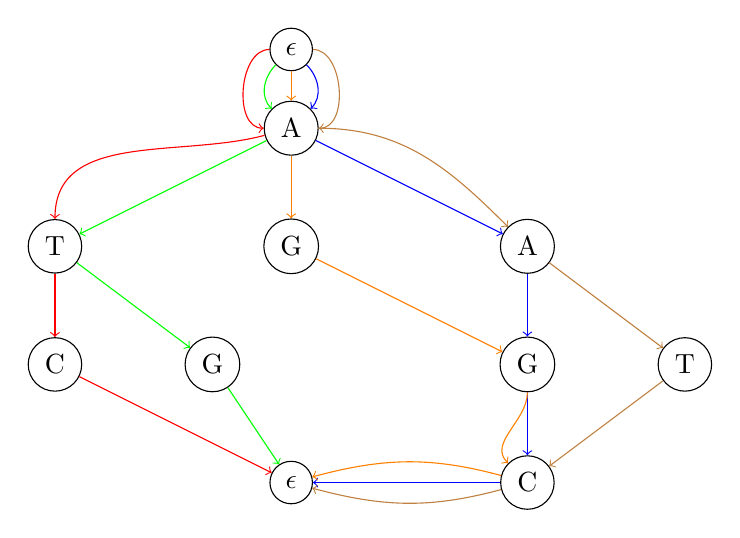
\begin{tikzpicture}
              % Nodi
              \node[draw, circle] (0) at (5, 1) {$\epsilon$};
              \node[draw, circle] (1) at (5,0) {A};
              \node[draw, circle] (2) at (2,-1.5) {T};
              \node[draw, circle] (3) at (8,-1.5) {A};
              \node[draw, circle] (4) at (2,-3) {C};
              \node[draw, circle] (5) at (4,-3) {G};
              \node[draw, circle] (6) at (8,-3) {G};
              \node[draw, circle] (7) at (8,-4.5) {C};
              \node[draw, circle] (8) at (5, -1.5) {G};
              \node[draw, circle] (10) at (10, -3) {T};
              \node[draw, circle] (12) at (5, -4.5) {$\epsilon$};
            
              % Archi
              \draw[red, ->] (0) to[out=180, in=180] (1);
              \draw[green, ->] (0) to[out=225, in=135] (1);
              \draw[orange, ->] (0) to[out=270, in=90] (1);
              \draw[blue, ->] (0) to[out=315, in=45] (1);
              \draw[brown, ->] (0) to[out=0, in=0] (1);

              \draw[green, ->] (1) -- (2);
              \draw[red, ->] (1) to[out=195, in=90] (2);
              \draw[blue, ->] (1) -- (3);
              \draw[brown, ->] (1) to[out=0, in=135] (3);
              \draw[orange, ->] (1) -- (8);
              \draw[orange, ->] (8) -- (6);
              \draw[red, ->] (2) -- (4);
              \draw[green, ->] (2) -- (5);
              \draw[blue, ->] (3) -- (6);
              \draw[blue, ->] (6) -- (7);
              \draw[orange, ->] (6) to[out=270, in=135] (7);
              \draw[brown, ->] (3) -- (10);
              \draw[brown, ->] (10) -- (7);
              \draw[blue, ->] (7) -- (12);
              \draw[brown, ->] (7) to[out=195, in=345] (12);
              \draw[orange, ->] (7) to[out=165, in=15] (12);
              \draw[red, ->] (4) -- (12);
              \draw[green, ->] (5) -- (12);
              
            \label{graph:variation-graph}
        \end{tikzpicture}
        \caption{Esempio di \textbf{grafo di variazione canonico}: ogni \emph{percorso} è rappresentato da un colore diverso.}
    \end{figure}

\subsection{Allineamento tra un grafo di variazione e una sequenza}
    E' possibile estendere ulteriormente le equazione di \textbf{Needleman-Wunsch} generalizzate a \textbf{grafi di sequenza} (\ref{equation:poa}) per adattarle all'utilizzo di \textbf{grafi di variazione}. In particolare, è necessario aggiungere un'ulteriore dimensione alla \emph{matrice di programmazione dinamica}, in modo da poter riuscire a memorizzare l'allineamento ottimo per ciascun cammino. Considerando un \textbf{grafo di variazione} $G = (V, E, \delta, P)$, questo viene espresso tramite le seguenti \emph{equazioni}:
     \begin{equation}
        M[v, j, p] = \max \begin{cases}
            M[u, j, p] + d(\delta(v), -) & \\
            M[u, j - 1, p] + d(\delta(v), x_j) & \\
            M[v, j - 1, p] + d(-, x_j) & \\
        \end{cases}
    \label{equation:variation-graph}
    \end{equation}
    $$\forall u \, s.t. \, (u,v) \in E, \, \forall j > 0, \, \forall p \in P $$
    \vspace{10pt}
     e dalle seguenti \emph{condizioni al contorno}:
\subsubsection{Caso globale}
    \textbf{Caso base}:
    \begin{equation}
        M[v, j, p] = \begin{cases}
            0 & v = v_0, \, j = 0 \\
            M[u, 0, p] + d(\delta(u), -)& \forall (u, v) \in E, \, j = 0 \\
            M[v_0, j - 1, p] + d(-, x_j)& v = v_0, \, j > 0
        \end{cases}
    \end{equation}
    $$\forall p \in P$$

    \textbf{Soluzione ottima}: $$\max_{p \in P} M[v_n, m, p]$$
    
\subsubsection{Caso semiglobale}
    \textbf{Caso base}:
    \begin{equation}
        M[v, j, p] = \begin{cases}
            0 & \forall v \in V, \, j = 0 \\
            M[v_0, j - 1, p] + d(-, x_j) & v = v_0, \, j > 0
        \end{cases}
    \end{equation}
    \textbf{Soluzione ottima}:
    $$\max_{v \in V, \, p \in P} M[v, m, p]$$

\subsubsection{Esempio}
A seguire un esempio grafico dell'\emph{allineamento} tra un \textbf{grafo di variazione} e una \textbf{sequenza}:
\begin{figure}[ht]
        \centering
        \begin{tikzpicture}
              % Nodi
              \node[draw, circle] (0) at (5, 1) {$\epsilon$};
              \node[draw, circle] (1) at (5,0) {A};
              \node[draw, circle] (2) at (2,-1.5) {T};
              \node[draw, circle] (3) at (8,-1.5) {A};
              \node[draw, circle] (4) at (2,-3) {C};
              \node[draw, circle] (5) at (4,-3) {G};
              \node[draw, circle] (6) at (8,-3) {G};
              \node[draw, circle] (7) at (8,-4.5) {C};
              \node[draw, circle] (8) at (5, -1.5) {G};
              \node[draw, circle] (10) at (10, -3) {T};
              \node[draw, circle] (12) at (5, -4.5) {$\epsilon$};

              \node[draw, circle] (x0) at (13, 1) {-};
              \node[draw, circle] (x1) at (13, 0) {A};
              \node[draw, circle] (x2) at (13, -1.5) {A};
              \node[draw, circle] (x3) at (13, -3) {G};
              \node[draw, circle] (x4) at (13, -4.5) {T};
              \node[draw, circle] (x5) at (13, -6) {-};
            
              % Archi
              \draw[red, ->] (0) to[out=180, in=180] (1);
              \draw[green, ->] (0) to[out=225, in=135] (1);
              \draw[orange, ->] (0) to[out=270, in=90] (1);
              \draw[blue, ->] (0) to[out=315, in=45] (1);
              \draw[brown, ->] (0) to[out=0, in=0] (1);

              \draw[green, ->] (1) -- (2);
              \draw[red, ->] (1) to[out=195, in=90] (2);
              \draw[blue, ->] (1) -- (3);
              \draw[brown, ->] (1) to[out=0, in=135] (3);
              \draw[orange, ->] (1) -- (8);
              \draw[orange, ->] (8) -- (6);
              \draw[red, ->] (2) -- (4);
              \draw[green, ->] (2) -- (5);
              \draw[blue, ->] (3) -- (6);
              \draw[blue, ->] (6) -- (7);
              \draw[orange, ->] (6) to[out=270, in=135] (7);
              \draw[brown, ->] (3) -- (10);
              \draw[brown, ->] (10) -- (7);
              \draw[blue, ->] (7) -- (12);
              \draw[brown, ->] (7) to[out=195, in=345] (12);
              \draw[orange, ->] (7) to[out=165, in=15] (12);
              \draw[red, ->] (4) -- (12);
              \draw[green, ->] (5) -- (12);

              \draw[dashed] (x0) to[out=165, in=90] (0);
              \draw[dashed] (x1) -- (1);
              \draw[dashed] (x2) -- (3);
              \draw[dashed] (x3) to[out=180, in=45] (6);
              \draw[dashed] (x4) -- (7);
              \node (x) at (10.5, -4.5) {\textbf{X}};
              \draw[dashed] (x5) to[out=165, in=270] (12);
              
            \label{graph:variation-graph-alignment}
        \end{tikzpicture}
        \caption{Esempio di allineamento tra un \textbf{grafo di variazione canonico} e una \textbf{sequenza}: il \emph{percorso ottimale} risulta essere quello blu.}
    \end{figure}
\subsubsection{Complessità computazionale}
\label{section:variation-complexity}
   A differenza dell'allineamento con un \textbf{grafo di sequenza} (sezione \ref{section:poa-complexity}), ogni vertice possiede un unico \emph{predecessore} e quindi, sebbene non immediatamente evidente dall'equazione \ref{equation:variation-graph}, ogni cella della matrice viene computata in $O(1)$ (come nell'allineamento tra sequenze). E' tuttavia necessario aggiungere la dimensione relativa ai \emph{percorsi} del grafo alla stessa matrice, che dunque assume una dimensione totale $(n+1) \times (m+1) \times k$, dove $k = \lvert P \rvert$. Di conseguenza, la \textbf{complessità in tempo} risulta essere:
    \begin{equation*}
        T(n, m, k) = O(n \cdot m \cdot k)
        \label{equation:variation_time_complexity}
    \end{equation*}
    
    Per quanto riguarda la \textbf{complessità in spazio}, ogni elemeneto della matrice continua a mantenere una quantità \emph{costante} di informazione: di conseguenza, essa è uguale a
    \begin{equation*}
        M(n, m, k) = O(n \cdot m \cdot k)
    \end{equation*}

\section{Allineamento con ricombinazione}
    Uno dei processi biologici che viene osservato con molta frequenza durante le fasi di duplicazioni del DNA sono le \textbf{ricombinazioni}, le quali consistono nell'importazione totale o parziale di geni al posto di materiale genetico presente in regioni omologhe a quelle importate del genoma di interesse. Uno degli organismi in cui risulta più interessante lo studio delle ricombinazioni sono i \emph{batteri}, nei quali questi processi avvengono con elevate frequenze: esse sono infatti state notate per la prima volta durante lo studio dei emph{loci batterici} che codificano per \emph{antigeni} o per \emph{resistenze agli antibiotici}.
    
    \vspace{20pt}
    Risulta interessante un approccio computazionale che estenda l'allineamento tra un \textbf{grafo di variazione} e una \textbf{sequenza} per riuscire a individuare una, o eventualmente più \textbf{ricombinazioni} avvenute all'interno del genoma rappresentato nel grafo: una trattazione approfondita dell'argomento è riportata in \cite{Recgraph}, mentre di seguito vengono riportate le idee principali dietro a questo tipo di allineamento.

\subsection{Definizioni}
    Si considera un \textbf{grafo di variazione canonico} $G = <V, E, \delta, P>$ (sezione \ref{section:variation_graph});
    
    si definiscono:
    \begin{itemize}
        \item una \textbf{ricombinazione} di \textbf{due percorsi} come una quadrupla $R = <p_1, p_2, \rho, \psi>$, dove 
            \begin{itemize}
                \item $p_1, p_2 \in P$ sono due \emph{cammini} del grafo;
                \item $\rho \in p_1$ e $\psi \in p_2$ sono due \emph{vertici} dei cammini selezionati.
            \end{itemize}

        \item i due vertici\footnote{Quando chiari dal contesto, i cammini $p_1, p_2$ e i vertici $\rho, \psi$ vengono omessi e i vertici indicati come $\alpha$ e $\beta$.} $\alpha_{p1, p2}(\rho, \psi) \in V$ e $\beta_{p1, p2}(\rho, \psi) \in V$ come due nodi per i quali:
        \begin{itemize}
            \item $\alpha_{p1, p2}(\rho, \psi)$ precede $\rho$ in $p_1$ e $\psi$ in $p_2$, e segue qualsiasi altro vertice $u$ che precede entrambi $\rho$ in $p_1$ e $\psi$ in $p_2$;
            \item $\beta_{p1, p2}(\rho, \psi)$ segue $\rho$ in $p_1$ e $\psi$ in $p_2$, e precede qualsiasi altro vertice $v$ che segue entrambi $\rho$ in $p_1$ e $\psi$ in $p_2$;
        \end{itemize}
        ricordando il concetto \emph{Lower Common Ancestor (LCA)} di un albero;

        \item il \textbf{displacement di una ricombinazione} come la quantità 
        \begin{equation}
            D = \lvert \lvert a_1 \rvert - \lvert a_2 \rvert + 1 \rvert + \lvert \lvert b_1 \rvert - \lvert b_2 \rvert - 1 \rvert 
            \label{equation:displacement}
        \end{equation}
        dove:
        \begin{itemize}
            \item $a_1, \, a_2$ sono i \emph{sottopercorsi} che vanno rispettivamente da $\alpha$ a $\rho$ e da $\alpha$ a $\psi$;
            \item $b_1, \, b_2$ sono i \emph{sottopercorsi} che vanno rispettivamente da $\rho$ a $\beta$ e da $\psi$ a $\beta$;
        \end{itemize}
        che vuole misurare il \emph{peso} di una \textbf{ricombinazione};

        \item un \textbf{allineamento con ricombinazione} come la concatenazione di due allineamenti senza ricombinazione:
        \begin{itemize}
            \item il primo che riguarda il \emph{sottopercorso} $a_1$ e il \emph{prefisso} $Y[:j]$,
            \item il secondo che riguarda il \emph{sottopercorso} $b_2$ e il \emph{suffisso} $Y[j+1:]$,
        \end{itemize}
        dove $Y_m$ è la sequenza da allineare e $j \in \{1, ..., m\}$ la posizione della sequenza in cui avviene la \textbf{ricombinazione}. 
    \end{itemize}

    Un esempio delle definizioni introdotte è mostrato nella figura \ref{fig:recombination_definitions_example}.

    \vspace{20pt}
    \begin{figure}[H]
        \centering
        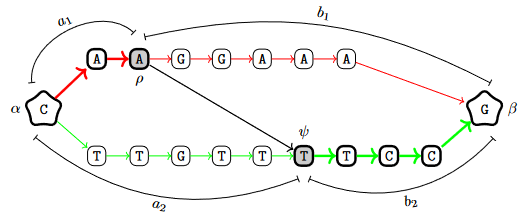
\includegraphics[width=1.0\linewidth]{images/recombination_definitions_example.png}
        \caption{Esempio di \textbf{displacement} di una \textbf{ricombinazione}. \cite{Recgraph}}
        \label{fig:recombination_definitions_example}
    \end{figure}

\subsection{Equazioni di ricorrenza}
    Come conseguenza della definizione, un \textbf{allineamento con ricombinazione} può essere computato attraverso due diversi \textbf{allineamenti senza ricombinazione}, uno che comprenda la porzione iniziale di un cammino e il prefisso della read e l'altro che si riferisca alla porzione finale di un altro cammino e al suffisso della stessa read.

    Formalmente, definita $M[v, j, p]$ come in \ref{equation:variation-graph} e $R[v, j, p]$ come il valore ottimale dell'allineamento globale tra la porzione finale di $p \in P$ che inizia nel vertice $\psi$ e tra il \emph{suffisso} $Y[:j]$, il valore ottimale dell'\textbf{allineamento con al più una ricombinazione} può essere descritto dalla ricorrenza \ref{equation:recombination}:

    \begin{equation}
        \max {\begin{cases}
            \max_{p \in P}{M[v_0, m, p]} & (a) \\
            \max_{(v, w), j, p \neq q}{M[v, j, p] + R[w, j+1, q] + d_o + d_e \cdot d(v,w)} & (b) \\
        \end{cases}}
        \label{equation:recombination}
    \end{equation}
    dove:
    \begin{itemize}
        \item $d(v, w)$ è il \textbf{displacement} tra $v$ e $w$ (equazione \ref{equation:displacement});
        \item $d_o$ è il \textbf{costo di apertura} del \textbf{displacement};
        \item $d_e$ è il \textbf{costo di estensione} del \textbf{displacement};
    \end{itemize}

    Se il massimo è verificato dal caso $(a)$, allora l' \emph{allineamento ottimale} è \textbf{senza ricombinazione}; se invece è verificato dal caso $(b)$, si trova un \textbf{allineamento con una ricombinazione}.

    \vspace{20pt}
    \begin{figure}[H]
        \centering
        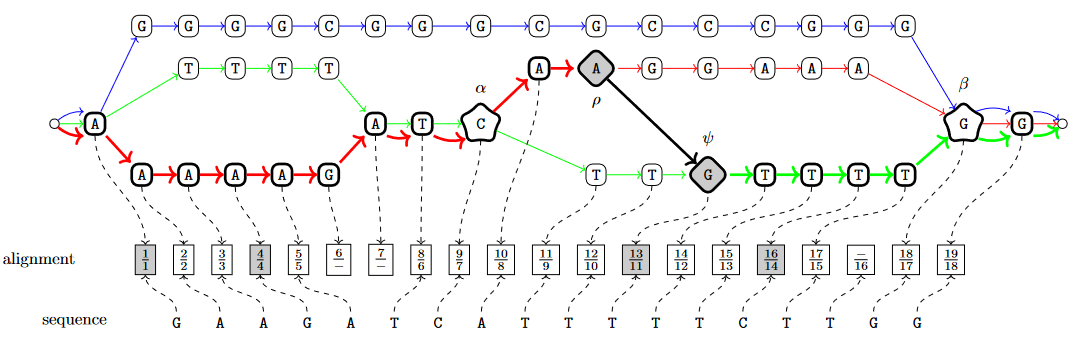
\includegraphics[width=1 \linewidth]{images/recombination_alignment.png}
        \caption{Esempio di un \textbf{allineamento ottimale con ricombinazione}. \cite{Recgraph}}
        \label{fig:recombination_alignment}
    \end{figure}
    

\subsection{Complessità computazionale}
\subsubsection{Complessità in tempo}
    La \textbf{complessità temporale} per computare le due matrici $M[v, j, p]$ e $R[v, j, p]$ rimane la stessa di \ref{equation:variation_time_complexity} (le due matrici possono anche essere calcolate in parallelo); di conseguenza, definiti
    \begin{itemize}
        \item $n = \lvert V \rvert$
        \item $m = \lvert Y \rvert$
        \item $p = \lvert P \rvert$
    \end{itemize}
    la \textbf{complessità in tempo} è data dal caso $(b)$ dell'equazione \ref{equation:recombination} e vale:

    \begin{equation}
        T(n, m, p) = O(n^2 \cdot m \cdot p^2)
        \label{equation:recombination_time_complexity}
    \end{equation}

\subsubsection{Complessità in spazio}
    Le due matrici $M[v, j, p]$ e $R[v, j, p]$ occupano la stessa quantità di memoria; di conseguenza la \textbf{complessità in spazio} rimane:

    \begin{equation}
        M(n, m, p) = O(n \cdot m \cdot p)
        \label{equation:recombination_space_complexity}
    \end{equation}

\subsection{RecGraph}
\label{section:recgraph}
    \href{https://github.com/AlgoLab/RecGraph}{\textbf{\textit{RecGraph}}} è un tool sviluppato dal laboratorio \href{https://algolab.eu/}{\textbf{BIAS}}, nel linguaggio di programmazione \href{https://www.rust-lang.org/it}{\textbf{\textit{Rust}}}, che permette di eseguire allineamenti tra un \textbf{grafo} e una \textbf{sequenza} in diverse modalità, tra cui la \textbf{\textit{recombination mode}}, in cui si cerca di individuare fino a una \textbf{ricombinazione} avvenuta nel genoma corrispondente a uno dei percorsi del grafo. Un'interessante ottimizzazione per l'allineamento su \textbf{grafi di variazione} implementata all'interno del tool è il \textbf{reference path}, che permette di evitare di calcolare più di una volta il valore dell'allineamento di vertici appartenenti a più di un \emph{cammino} (spiegazione formale contenuta in \cite{Recgraph}).    

    \vspace{20pt}
    L'obiettivo finale dello stage era quello di cercare di migliorare le capacità computazionali di \textbf{\textit{RecGraph}}, concentrandosi sull'allineamento tra un \textbf{grafo di variazione} e una \textbf{sequenza}, in maniera che potesse poi essere utilizzato nella \textbf{\textit{recombination mode}} su grafi di dimensioni maggiori (e, in futuro, possa essere usato per permettere più di una ricombinazione): per far questo, si è passati allo studio dell' \textbf{algoritmo \textit{wavefront}}, di cui segue una trattazione formale nel capitolo successivo.